\chapter{Introducción}
\label{chp:introduccion}
%\pdfbookmark{Introducción}{int}
%\pdfbookmark{\contentsname}{Introduccion}

Una vez concluida la producción primaria en yacimientos de petróleo, la mayor parte del fluido se encuentra aún en el yacimiento. A partir de este punto se requieren de otros métodos para poder recuperar de forma eficiente el fluido remanente. Otros fluidos como gua o gas pueden ser inyectados para aumentar la presión existente en el yacimiento.

A la conversión de algunos pozos productores a inyectores y la subsecuente inyección de gas o agua para mantener la presión en el yacimiento se le conoce como recuperación secundaria. Históricamente la recuperación terciaria o mejorada (\textbf{EOR}) se ha referido a una tercera etapa de producción, donde se pueden aplicar gases de forma miscible, productos químicos o energía térmica para desplazar aceite adicional una vez que la recuperación secundaria llega a su límite económico; sin embargo, se podría definir simplemente como cualquier proceso de recuperación aplicado después de la recuperación secundaria (\cite{Lake}).

Se ha reportado que aun después de la recuperación primaria y secundaria, la saturación de aceite residual típica en yacimientos de aceite ligero se encuentra en el rango de $50$ a $60$ \% del volumen original (\cite{Moritis}). Esta baja eficiencia en la recuperación es causada principalmente por la heterogeneidad en el yacimiento, que controla la distribución espacial de la porosidad y la permeabilidad, por ello incrementar el factor de recuperación es uno de los grandes retos hoy en día en la industria petrolera (\cite{Alvarado}).


\section{Inyección de agentes químicos}

Como se mencionó, existen diversos métodos para la recuperación de hidrocarburos: la inyección de productos químicos como polímeros y surfactantes, métodos térmicos (estimulación con vapor de agua y combustión \textit{in-situ} ), inyección de gases miscibles, así como procesos microbiológicos eléctricos y vibracionales, (\cite{Ali1996}) .

Uno de los métodos más convenientes para resolver los complejos problemas presentados durante la recuperación de aceite crudo, es el uso de agentes químicos, debido a sus ventajas operativas y económicas, dado que implica pocos cambios en los proceso normales de operación (\cite{Sheng2010}).

\subsection{Inyección de surfactantes}

El uso de surfactantes ha sido por mucho tiempo considerado como uno de los principales métodos para incrementar la recuperación de crudo. Los principales mecanismos de acción inducidos por el uso de surfactantes son: el cambio en la mojabilidad y la reducción de tensión interfacial entre agua y aceite (\cite{Austad1998}, \cite{Hirasaki2004} y \cite{Standnes2000}).

Hoy en día, los surfactantes convencionales tienen en un amplio rango de aplicaciones, y son comúnmente usados para la estimulación matricial y el fracturamiento hidráulico (\cite{Sullivan2006}).

La habilidad de los surfactantes para formar micelas, les concede propiedades viscoelásticas que han sido aprovechadas en la industria petrolera para controlar la mobilidad de fluidos en el yacimiento (\cite{LaastreBuelvas2012}).

\section{Problemática y propuesta de solución}

Un corte de agua excesivo en el intervalo productor es una de las dificultades mas grandes para sostener el ritmo de producción en los pozos. Algunos pozos del campo Cantarrell, que es un campo maduro depresionado ubicado en la bahía de Campeche en el golfo de México, atraviesan por un decremento drástico en su producción y, dependiendo de la zona productora, un incremento en la producción de agua y/o gas. Este incremento del corte de agua tiene un fuerte impacto sobre la estrategia de producción (\cite{Lopez2014}).

Entre los problemas asociados con la producción excesiva de agua y gas están la corrosión y la formación de depósitos en tuberías. La producción excesiva de agua puede además implicar costos adicionales por el manejo y penalizaciones de tipo contractual (\cite{Bailey2000}). El agua producida en yacimientos maduros puede contener sustancias como arsénico, mercurio y otras sales que pueden dañar severamente el ambiente si no son dispuestas de manera correcta (\cite{Hibbeler2005}). La producción excesiva de agua requiere de un técnica de remediación que permita reducir o bloquear la fuente de agua hacia el pozo. La inyección de geles poliméricos se encuentra entre uno de los métodos mas comunes para atacar este problema (\cite{ElKarsani2015}).

Se ha demostrado que la inyección de un surfactante viscoelástico puede disminuir considerablemente el corte de agua y aumentar la producción de aceite. Los surfactantes zwitterionicos se encuentran dentro de las especies de surfactantes efectivos en aplicaciones de control de movilidad (\cite{Lakatos2007} y \cite{LaastreBuelvas2012}).

Las soluciones de surfactantes son capaces de formar fases ordenadas y desordenadas compuestas por una gran variedad de estructuras auto ensambladas supramoleculares. La organización de estas estructuras supramoleculares depende de la complejidad de las interacciones entre geometría, carácter ambifílico y carga de las moléculas involucradas. Estas interacciones pueden modificarse por muchos factores como la concentración del surfactante, hidrotropia de las sales, pH y fuerza iónica del medio en el que se encuentran (\cite{LopezDiaz2010}).

Algunos autores (\textcolor{Green}{Zamudio et al., 2017 inédito}) han planteado el emplazamiento en la formación de una estructura supramolecular \textbf{organogel} impermeable al agua congénita pero permeable al aceite mediante de la inyección de un surfactante viscoelástico de tipo zwitteriónico. Dicho organogel provee una solución al control de movilidad de fluidos en formaciones carbonatadas y con zonas de alta conductividad como yacimientos naturalmente fracturados así como aprovecha el carácter electrostático de estas moléculas para inhibir la formación de depósitos inorgánicos, prevenir la corrosión, evitar el depósito de asfaltenos a la vez que altera la mojabilidad de la roca. 

%La efectividad del mecanismo de reducción en la tensión interfacial (\textbf{IFT}), está
%condicionado por el hecho de que el surfactante debe ser capaz de reducir la tensión
%interfacial entre agua y aceite, de $4$ a $6$ órdenes de magnitud, por lo que generalmente se requiere de la inyección de agua con una salinidad óptima, para alcanzar esta reducción
%en la \textbf{IFT} (\cite{Iglauer2010} y \cite{Snchez2014}).
%
%Los agentes químicos capaces de lograr el efecto deseado son caros y se necesitan
%grandes cantidades y concentraciones, por lo que no son económicamente factibles para
%su aplicación en campo (\cite{Sheng2010}, \cite{Hirasaki2004}).
%Por lo anterior nuevas moléculas de agentes surfactantes, que son capaces de alterar las
%condiciones de mojabilidad, en concentraciones moderadas, son de gran interés para las
%operaciones de recuperación.

\subsection{Líquidos Zwitteriónicos}

Los líquidos zwitteriónicos ({\textbf LZ}), son considerados dentro de las especies moleculares
utilizadas para la recuperación mejorada (\cite{LpezChvez2012}, \cite{altamirano2013}). La estructura molecular de los \textbf{LZ} está constituida por dos cadenas de
hidrocarburos, un puente y dos grupos polares de tipo zwitteriónico. Los \textbf{LZ} son
compuestos que contienen un catión y un anión en diferentes átomos de la misma
molécula, lo que los hace eléctricamente neutros y les concede la oportunidad de
comportase como ácidos o bases (donador o receptor), de acuerdo con las características
del ambiente en el que se encuentren. Esto significa, que estas moléculas (\textbf{LZ}) se comportan como modificadores “inteligentes” de la mojabilidad, que pueden responder de manera eficiente dependiendo de las características de uno o varios ambientes específicos en los que se encuentren (\cite{LpezChvez2012}).

\begin{figure}

\centering

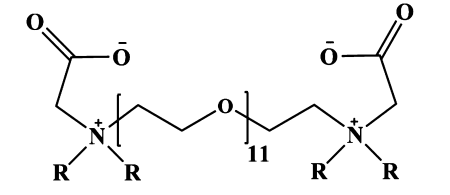
\includegraphics[width=0.7\textwidth]{Graphics/ZLZamudio.png}

\caption[Molécula zwitterion propuesta]{Estructura general de la molécula zwitteriónica propuesta por (\cite{AlczarVara2015}).}

\label{fig:ZLZamudio}

\end{figure}


En este trabajo se presenta el estudio experimental sobre el desempeño a través de sus propiedades de una nueva clase de líquido zwitteriónico, como agente surfactante para la recuperación avanzada.
La estructura química más general del \textbf{LZ} utilizado en este trabajo se muestra en la \autoref{fig:ZLZamudio}, esta molécula pertenece a un desarrollo reciente de surfactante geminal zwitteriónico alquilbetaino con espaciadores de polietileno (\cite{AlczarVara2015}).


%\section{Motivación}
%
%\section{Distribución del aceite en yacimientos}

%Como es un yacimiento (fracturados, múltiple porosidad )
%Como se distribuye el aceite y el agua
%Formación de emulsiones naturales (presencia de agua, )
%Surfactantes
%Los efectos descritos anteriormente pueden ser controlados por medio de la inyección de químicos al yacimiento. A continuación se describen los principales producto utilizados de manera comercial para este fin.
% naturales (resinas y los asfaltenos)
%
%Dado que se tienen lo dos fluidos en contacto, que pueden emulsionarse o separarse, pueden ocurrir diversos escenarios, como la producción de crudo emulsionado, el incremento en la cantidad de agua en la producción debido a l fenomeno conocido como canalización (ref) o la formación de precipitados de sales inorgánicas.



\section{Objetivos}
\begin{description}
\item[General] Proponer un mecanismo para la formación de un organogel formado por la interacción de un surfactante zwitteriónico, agua congénita y aceite provenientes de un yacimiento mexicano, utilizado para la recuperación mejorada de crudo, en base a la determinación de propiedades reológicas, estabilidad de las fases formadas, tiempos de drenado y tensión interfacial.

\clearpage

\item[Específicos] \hfill
  \begin{itemize}
    \item \textbf{Evaluar} el drenado del organogel, durante el reposo a temperatura controlada.
    \item \textbf{Determinar} los parámetros de medición, que permitan mejorar la repetividad en las mediciones reológicas.
    \item \textbf{Correlacionar} las propiedades reológicas con la morfología de las fases obtenida mediante microscopía óptica. 
    \item \textbf{Medir} la tensión superficial y tensión interfacial para las fases presentes en el sistema para su posible correlación con el comportamiento reológico.
    %\item \textbf{Determinar} el contenido de agua del organogel y su relación con la concentración de producto químico.
  \end{itemize}
 
%\section{Metas}
 
%\item[Metas] Como metas específicas del trabajo están la publicación de un artículo técnico en una revista científica, así como la defensa del trabajo de tesis para obtener el grado de maestría.
\end{description}
%
%\section{Contenido de la tesis}